\documentclass{beamer}
\usetheme{Singapore}

\usepackage{listings}
\usepackage{booktabs}
\usepackage{amssymb}                 %extended symbols
\usepackage{amsmath}                 %misc math formatting
\usepackage{algorithm}
\usepackage[noend]{algpseudocode}


\title[SIDH]{Efficiency of SIDH/Isogeny Signatures}
\author{Robert Gorrie}
\institute[Comp Sci 2S03]{Department of Computing \& Software, McMaster University}
\date{November 16th, 2017}

\begin{document}

\begin{frame}
\titlepage
\end{frame}

\begin{frame}
\frametitle{Table of Contents}
\tableofcontents
\end{frame}

\AtBeginSection[]{
\begin{frame}<beamer>
\frametitle{Table of Contents}
\tableofcontents[currentsection]
\end{frame}
}

\section{Isogeny Based Signatures}

%high level signature description via fiat-shamir

\begin{frame}
\frametitle{Current Performance of SIDH}
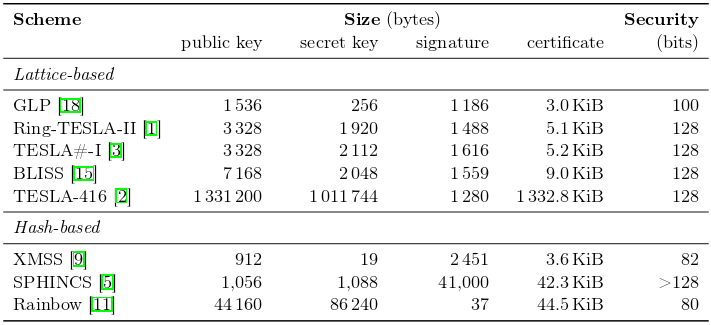
\includegraphics[scale=0.43]{sigcomparison.png}
\end{frame}

\begin{frame}
\frametitle{Isogeny Based Signatures}
\begin{itemize}
\item Yoo et. al provide an isogeny based signature scheme built off the Microsoft SIDH 1.0 Library.
\item The scheme is constructed using the ZKPoI protocol provided in the original SIDH paper in tandem with Unruh's PQ secure Fiat-Shamir transform.
\item The scheme involves performing 248 (seperate) instances of SIDH key exchange with an arbitrary thirdparty
\item These instances are parallelizable but overall extremely computationally expensive
\end{itemize}
\end{frame}

\begin{frame}
\frametitle{Isogeny Signature Parameter Sizes}
\begin{tabular}{@{}lllll@{}}
	Scheme & Public-key size & Private-key size & Signature size\\
	\midrule
	Hash-based & 1,056 & 1,088 & 41,000\\
	Code-based & 192,192 & 1,400,289 & 370\\
	Lattice-based & 7,168 & 2,048 & 5,120\\
	Ring-LWE-based & 7,168 & 4,608 & 3,488\\
	Multivariate-based & 99,100 & 74,000 & 424\\
	\midrule
	Isogeny-base & 768 & 48 & 141,312\\
\end{tabular}\\
\end{frame}

\section{Inversion Batching}

%slide with each main point/part of the procedure 3 slides

%before this, background on inversions in sidh/sig
\begin{frame}[fragile]
\frametitle{Partial Inversion Procedure}
%\begin{algorithm} center with input and output
\begin{algorithmic}[1]
	\State $t_0 \gets a_{0}^{2}$
	\State $t_1 \gets a_{1}^{2}$
	\State $den \gets t_0 + t_1$
	\State $den \gets den^{-1}$
	\State $a_{0} \gets a_{0} * den$
	\State $a_{1} \gets a_{1} * den$
\end{algorithmic}
%\end{algorithm}
%equation for inverting two elements, shamir?
%operation count reduction
\end{frame}

\begin{frame}[fragile]
\frametitle{Batched Inversion Procedure}
If we combine these two procedures we can reduce $n$ $\mathbb{F}_{p^{2}}$ inversions to:
\begin{itemize}
\item $1$ $\mathbb{F}_{p}$ inversion
\item $3(n-1)$ $\mathbb{F}_{p}$ multiplications
\item $2n$ $\mathbb{F}_{p}$ multiplications
\item $2n$ $\mathbb{F}_{p}$ squarings
\end{itemize}
Or, roughly 1 $\mathbb{F}_{p}$ inversion and 7n $\mathbb{F}_{p}$ multiplications
\end{frame}

\begin{frame}[fragile]
\frametitle{Performance Increase}
The following are measured in billions of clock cycles
\begin{center}
\begin{tabular}{@{}lllll@{}}
	\toprule
	Procedure & Without Batching & With Batching\\
	\midrule
	Signature Sign & 15.74 & 15.56\\
	Sign Parallel & 10.23 & 10.13\\
	Signature Verify & 11.18 & 10.8\\
	Verify Parallel & 7.27 & 7.11\\
	\bottomrule
\end{tabular}\\
\end{center}
\begin{itemize}
\item In the serial setting we see a 1.1\% and a 3.5\% performance increase for Signing and Verifying, respectively.
\item Comparatively, in the parallel setting we see a 0.9\% and a 2.3\% performance increase.
\end{itemize}
\end{frame}

\section{Signature Compression}

\begin{frame}
\frametitle{SIDH Key Compression}
A recent paper from Microsoft Research showed that SIDH public keys could be compressed to 330 bytes while retaining 128 bits of security in the quantum setting.  
\end{frame}

\begin{frame}
%goal
\frametitle{Signature Compression}
\end{frame}

%preliminary results
\begin{frame}
\frametitle{Results}
\end{frame}

\section{Additional Work}

\begin{frame}
\frametitle{}

\begin{center}
%\includegraphics[scale=0.65]{code5.png}
\end{center}
\end{frame}

\end{document}
